%% This is file `DEMO-TUDaReport-de.tex' version 3.40 (2024-07-01),
%% it is part of
%% TUDa-CI -- Corporate Design for TU Darmstadt
%% ----------------------------------------------------------------------------
%%
%%  Copyright (C) 2018--2024 by Marei Peischl <marei@peitex.de>
%%
%% ============================================================================
%% This work may be distributed and/or modified under the
%% conditions of the LaTeX Project Public License, either version 1.3c
%% of this license or (at your option) any later version.
%% The latest version of this license is in
%% http://www.latex-project.org/lppl.txt
%% and version 1.3c or later is part of all distributions of LaTeX
%% version 2008/05/04 or later.
%%
%% This work has the LPPL maintenance status `maintained'.
%%
%% The Current Maintainers of this work are
%%   Marei Peischl <tuda-ci@peitex.de>
%%
%% The development respository can be found at
%% https://github.com/tudace/tuda_latex_templates
%% Please use the issue tracker for feedback!
%%
%% If you need a compiled version of this document, have a look at
%% http://mirror.ctan.org/macros/latex/contrib/tuda-ci/doc
%% or at the documentation directory of this package (if installed)
%% <path to your LaTeX distribution>/doc/latex/tuda-ci
%% ============================================================================
%%
% !TeX program = lualatex
%%

\documentclass[
	german,
	accentcolor=9c,% Farbe für Hervorhebungen auf Basis der Deklarationen in den
	type=intern,
	marginpar=false
	]{tudapub}

\usepackage[english]{babel}
\usepackage[autostyle]{csquotes}
\usepackage{graphicx}               % Required for inserting images
\usepackage{amsmath}                % Required for equations
\usepackage{booktabs}                % Required for tables
\usepackage{url}
\usepackage{hyperref}
\usepackage{xcolor}

\usepackage{siunitx}
\usepackage[version=4]{mhchem}

%%%%%%%%%%%%%%%%%%%%%%%%%%%%%%%%%%%%%%%%%%
% Uncomment to change font
%\usepackage{lmodern}
%\renewcommand{\familydefault}{\sfdefault}
%%%%%%%%%%%%%%%%%%%%%%%%%%%%%%%%%%%%%%%%%%

\linespread{1.6}

%Formatierungen für Beispiele in diesem Dokument. Im Allgemeinen nicht notwendig!
\let\file\texttt
\let\code\texttt
\let\pck\textsf
\let\cls\textsf

\begin{document}

\title{Title}
\author{Author}
%\date{} % Ohne Angabe wird automatisch das heutige Datum eingefügt

\maketitle

\tableofcontents

\newpage

\section{Task description}
In this task, you will write a LaTeX report using the official TU template about your data analysis of the Spotify dataset. 

\begin{itemize}
\item Don’t worry: you are not expected to write extensive text about music theory. You may keep your responses concise, as long as they fully address the questions. Your report will be evaluated on a technical basis, focusing on whether it adheres to the basic rules of scientific reporting (see Section \ref{marking_guide}). 

\item For your convenience, these guidelines are summarized below as a tutorial and also serve as the initial LaTeX template. Please read them carefully and examine the commands used in the raw file (visible on the left side of the screen).

\item Your final report should not include any text from this template. Instead, replace all placeholder content with your solutions to the tasks, as you would in a real lab report. Feel free to use sections, subsections, and other structural elements, as long as they are logical and contribute to the clarity and organization of your report.
\end{itemize}


\subsection{Guidelines}       % Start a new subsection within the section

\subsubsection{Equations}  % Start a new subsubsection

Equations should be formatted with \LaTeX\,\href{https://www.overleaf.com/learn/latex/Learn_LaTeX_in_30_minutes#Adding_math_to_LaTeX} {\textcolor{blue}{(Link to tutorial)}}. 

\paragraph{Formatting non-mathematical text}         % Start a new paragraph 
Some mathematical functions--such as trigonometric functions, logarithmic functions, and exponential functions--are treated as text operators rather than simple variables. These functions are predefined in LaTeX and must be formatted correctly to distinguish them from ordinary variables or symbols.
Without the backslash, LaTeX assumes these are variables rather than recognized functions, formatting them in italics by default. This can make mathematical expressions harder to read and cause confusion (Table \ref{tab:functions}).

Sometimes, normal text needs to appear in math mode, such as units or specific labels. In such cases, use \texttt{mathrm} to ensure upright text.
Using \texttt{mathrm} ensures that non-mathematical text, such as units or labels, appears in the correct typographical style. \emph{Hint: you find an automated and more consistent way to typeset numbers and their units in the file \texttt{siunitx-template}.}

\begin{table}[h!]
\centering
\begin{tabular}{lll}
\toprule
    &    Syntax & Rendering \\
\midrule
Correct & \verb|f(x) = \sin(x) + \ln(x) + \exp(x)| & $ f(x) = \sin(x) + \ln(x) + \exp(x) $  \\
Incorrect & \verb|f(x) = sin(x) + ln(x) + exp(x)| & $ f(x) = sin(x) + ln(x) + exp(x) $  \\
\midrule
Correct & \verb|v = 5 \, \mathrm{m/s}| & $ v = 5 \, \mathrm{m/s} $  \\
Incorrect & \verb|v = 5 \, m/s| & $ v = 5 \, m/s $  \\
\bottomrule
\end{tabular}
\caption{LaTeX math syntax and rendering of mathematical and non-mathematical text.}
\label{tab:functions}
\end{table}

As shown in Equation \eqref{eq:reaction}, also equations can (and should) be labelled and referenced in the main text. See the usage of the commands \texttt{label} and \texttt{ref} within this text.

\begin{equation}
\mathrm{A + B \longrightarrow C + D}
\label{eq:reaction}
\end{equation}


\subsubsection{Tables}  % Start a new subsubsection

Tables should be used when the data cannot be presented clearly in the narrative, when many numbers must be presented, or when more meaningful inter-relationships can be conveyed by the tabular format. Tables should supplement, not duplicate, information presented in the text and figures. 

\begin{itemize}  
\item Tables should be simple and concise without overuse of horizontal and (especially) vertical lines.
\item All tables should be labelled. See the usage of the command \texttt{label} in Table \ref{tab:functions}.
\item All tables should be explicitly referenced in the main text. See the usage of the command \texttt{ref} within this text.
\item All tables should be accompanied by captions. Captions should be self-contained and provide sufficient information to be understood independently of the main text.
\end{itemize}

\subsubsection{Figures}  % Start a new subsubsection

\begin{itemize}                     % Start an itemized (bulleted) list
\item Figures should exhibit an appropriate size and aspect ratio. All figures throughout the report should exhibit consistent formatting. 
As a general guideline, the text within a figure should be similar in size to the text in the main body of the document. You may re-plot a figure in your Jupyter Notebook as needed until you are satisfied with its aspect ratio and font size. Play around with \texttt{width} to scale the figure in relation to the page width \href{https://www.overleaf.com/learn/latex/Inserting_Images#Changing_the_image_size_and_rotating_the_picture}{(see how it is done in Figure \ref{fig:bad} and \ref{fig:good}, and look at the \textcolor{blue}{tutorial})}. \emph{Welcome to the real world of paper writing.} Hint: Once you identify the settings that work best for you, apply them consistently to all subsequent figures to maintain a uniform appearance throughout the document.
    \begin{itemize}          
    \item Figure \ref{fig:bad} shows a bad example: the figure is unnecessarily large. 
    \item Figure \ref{fig:good} exhibits an appropriate size and the text size is comparable to the main text.
    \end{itemize}  
\item All figures should be labelled \href{https://www.overleaf.com/learn/latex/Learn_LaTeX_in_30_minutes#Captions,_labels_and_references}{(See the usage of the command \texttt{label} in Figure \ref{fig:bad} and \ref{fig:good}, and look at the \textcolor{blue}{tutorial})}.
\item All figures should be explicitly referenced in the main text. See the usage of the command \texttt{ref} within this text.
\item All figures should be accompanied by captions. Captions should be self-contained and provide sufficient information to be understood independently of the main text.
    \begin{itemize}                    
    \item The caption of Figure \ref{fig:bad} is not informative. 
    \item The caption of Figure \ref{fig:good} is informative.
    \end{itemize}  
\end{itemize}                       % End of the itemized list


\begin{figure}[htbp]         % 'h' means place the figure here                     
\centering                                              % Center the figure
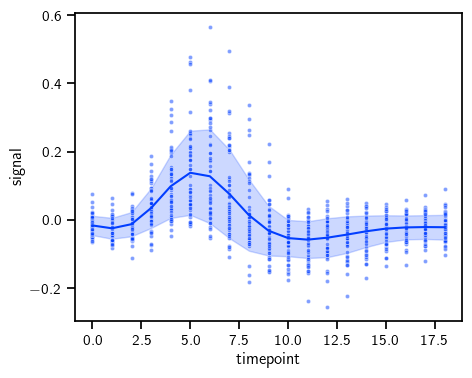
\includegraphics[width=\textwidth]{output.png} % Include an image with specified width
\caption{Signal against timepoint.}                         % Caption for the figure
\label{fig:bad}                                      % Label for referencing the figure
\end{figure}                                           % End of the figure environment

\begin{figure}[h]                                    % 'h' means place the figure here
\centering                                              % Center the figure
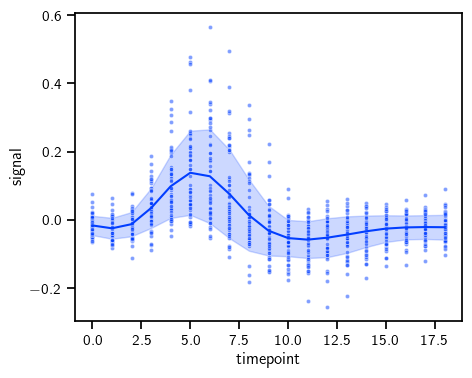
\includegraphics[width=0.6\textwidth]{output.png} % Include an image with specified width
\caption{FMRI signals as a function of time. Individual data points are represented as a scatter plot. At each time point, multiple measurements are aggregated through their mean (continuous line) and standard deviation (shaded area).}                         % Caption for the figure
\label{fig:good}                                      % Label for referencing the figure
\end{figure}                                           % End of the figure environment

%\clearpage

\subsubsection{Things you might find helpful in the future}  % Start a new subsubsection
\begin{itemize}
\item Refer to the file \texttt{siunitx-template} to learn how to correctly typeset numbers and their units.
\item \href{https://www.overleaf.com/learn/latex/Chemistry_formulae#Using_mhchem_to_typeset_chemical_formulae_and_equations}{\textcolor{blue}{Typesetting of chemical formulae and equations}}.
\end{itemize}

\clearpage

\section{Tasks}       % Start a new subsection within the section

\begin{itemize}
\item Read all the guidelines: they contain instructions, hints, and help. 
\item Read them again.
\item If in the previous assignment you received comments, this is the moment to address them.
\end{itemize}

\subsection{}
\begin{itemize}
\item Briefly describe the dataset: how many columns does it have?
\item In your notebook, paste and execute the following snippet:
\end{itemize}

\begin{verbatim}
data = {
    "Header": [
        "Title", "Artist", "Year", "Acousticness", "Danceability", 
        "Energy", "Instrumentalness", "Loudness, dB", "Speechiness", 
        "Tempo", "Valence", "Popularity", "Explicit", "Duration, minutes"],
    "Description": [
        "The title of the track.", 
        "The name of the artist or band.",
        "The Year the track was released.",
        "A score representing the likelihood that the track is acoustic.",
        "A score that describes how suitable the track is for dancing.",
        "A score representing the intensity and activity of the track.",
        "A score estimating the amount of instrumental content (no vocals).",
        "The average loudness of the track in decibels (dB).",
        "A score indicating the presence of spoken words in the track.",
        "The tempo of the track in beats per minute (BPM).",
        "A score representing the positivity or 'happiness' of the track.",
        "A score indicating the track’s popularity based on streams and ratings.",
        "Whether or not the track has explicit lyrics.",
        "The duration of the track in minutes."]
}

headers = pd.DataFrame(data)

print(headers.to_latex(index=False))
\end{verbatim}

\begin{itemize}
\item Copy and paste the LaTeX output into this document and execute it to view the formatted result. Add a label and a caption to the table. Briefly describe the table in one sentence, referring to it properly by its label.
\end{itemize}

\subsection{}
\begin{itemize}
\item Insert the plot you created in Task 5 as a figure.
\item Ensure the figure is properly labeled and captioned, and include a brief description that references it correctly in the text.
\item What type of error bar is shown in this plot? Identify the formula used and include it in the document, ensuring proper formatting for non-mathematical text.
\end{itemize}

\subsection{}
\begin{itemize}
\item Insert the plots you created in Task 6 as two figures.
\item Ensure the figures are properly labeled and captioned. Include a brief description that references them correctly and reports the skewness value.
\end{itemize}

\subsection{}
\begin{itemize}
\item Insert the heatmap you created in Task 7 as a figure. 
\item Ensure the figure is properly labeled and captioned. Include a brief description that references it correctly and justifies your choice to plot Loudness vs.\,Energy in the next task. 
\end{itemize}

\subsection{}
\begin{itemize}
\item Insert the curve fitting you created in Task 8.3 as a figure. 
\item Ensure the figure is properly labeled and captioned. Include a brief description that references it correctly, as well as the equation you used for the fit. The equation should be correctly formatted accounting for the text operator $\log$.
\end{itemize}

\subsection{}
\begin{itemize}
\item Insert the plots you created in Task 9 as two figures. 
\item Ensure the figures are properly labeled and captioned. Include a brief description that references them correctly and reports the skewness value.
\item What type of error bar is shown in the bar plot? Identify the formula used and include it in the document, ensuring proper formatting for non-mathematical text.
\end{itemize}

\subsection{}
\begin{itemize}
\item Insert the plots you created in Task 10 as two figures. 
\item Ensure the figures are properly labeled and captioned. Include a brief description that references them correctly.
\item Create a table where each row represents the Explicit values (Yes and No), and the columns display the average popularity scores (one digit after the decimal point) for different time periods: Overall, Since 1980, Since 1990, Since 2000, and Since 2010.
\end{itemize}

\section{Marking guide}\label{marking_guide}
There are 17 points available in total: you need at least 12 points to pass.
Your assignment will be evaluated based on technical questions:
\begin{enumerate}
\item Do the figures maintain proper size and aspect ratio, including font size?
\item Are the figures correctly referenced in the text?
\item Are the figure captions informative and self-contained?
\item Are the tables correctly referenced in the text?
\item Are the table captions informative and self-contained?
\item Are the equations correctly formatted?
\item Are the equations correctly referenced in the text?
\end{enumerate}


\small
\begin{tabular}{cccccccccccc}
\toprule
 & Fig 1 & Fig 1 & Fig 1 & Fig 2 & Fig 2 & Fig 2 & Table & Table & Equation & Equation \\
  & Aesthetics & Reference & Caption & Aesthetics & Reference & Caption & Caption & Reference & Formatting & Reference \\
\midrule
Task 1 & - & - & - & - & - & - & 0.5 & 0.5 & - & - \\
Task 2 & 0.3 & 0.5 & 0.5 & - & - & - & - & - & 0.5 & 0.5 \\
Task 3 & 0.3 & 0.5 & 0.5 & 0.3 & 0.5 & 0.5 & - & - & - & - \\
Task 4 & 0.3 & 0.5 & 0.5 & - & - & - & - & - & - & - \\
Task 5 & 0.3 & 0.5 & 0.5 & - & - & - & - & - & 0.5 & 0.5 \\
Task 6 & 0.3 & 0.5 & 0.5 & 0.3 & 0.5 & 0.5 & - & - & 0.5 & 0.5 \\
Task 7 & 0.3 & 0.5 & 0.5 & 0.3 & 0.5 & 0.5 & 0.5 & 0.5 & - & - \\
\bottomrule
\end{tabular}

\end{document}
